\chapter{Лабораторная работа}

\section{Цель работы}

Целью лабораторной работы №1 является освоение возможностей программы Microsoft Project для планирования проекта по разработке программного обеспечения.

\section{Содержание проекта}

Команда разработчиков из 16 человек занимается созданием карты города на основе собственного модуля отображения. Проект должен быть завершен в течение 6 месяцев. Бюджет проекта: 50 000 рублей.

\section{Настройка рабочей среды проекта}

На вкладке \texttt{Проект -> Сведения о проекте} внесены параметры по условию.

\begin{figure}[H]
	\begin{center}
		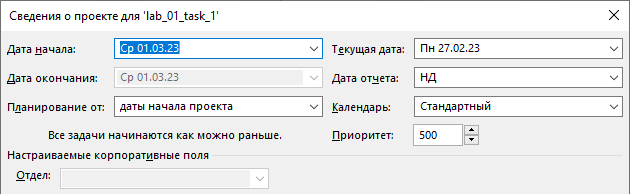
\includegraphics[scale=0.8]{imgs/task_1_0.png}
	\end{center}
	\caption{Настройка сведений о проекте}
	\label{img:label}
\end{figure}

На вкладке \texttt{Файл -> Параметры -> Расписание} установлены параметры рабочей недели и планирования.

\begin{figure}[H]
	\begin{center}
		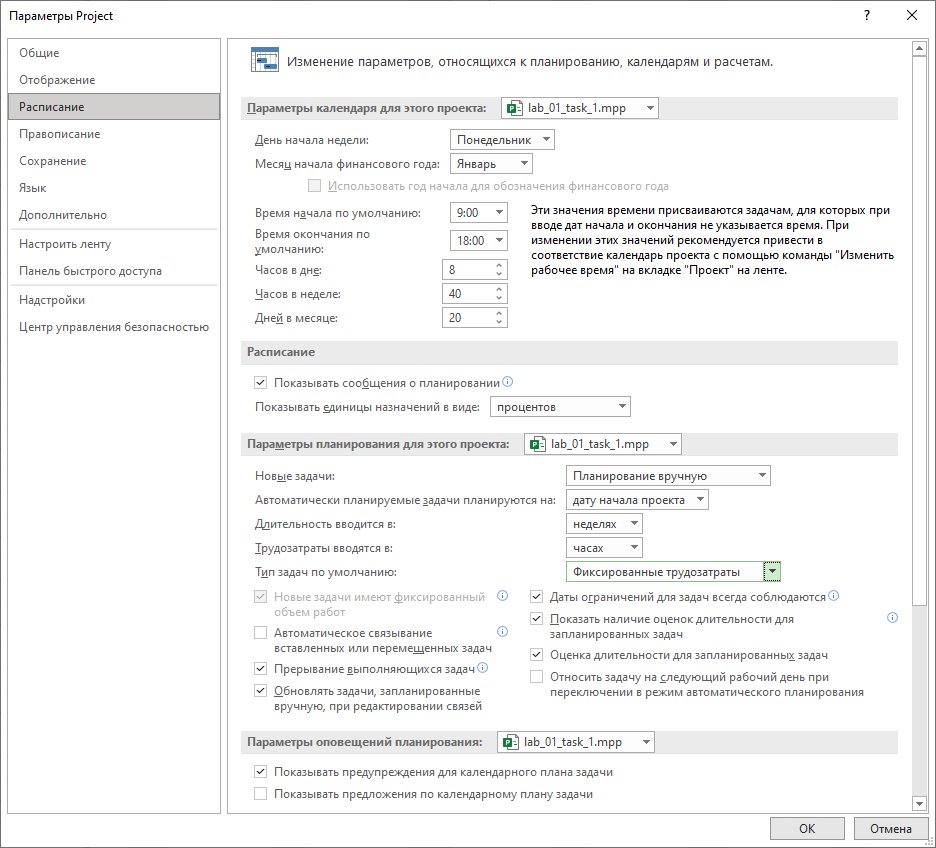
\includegraphics[width=\textwidth]{imgs/task_1_1.png}
	\end{center}
	\caption{Настройка расписания}
	\label{img:label}
\end{figure}

На вкладке \texttt{Проект -> Изменить рабочее время} установлены нерабочие праздничные дни.

\begin{figure}[H]
	\begin{center}
		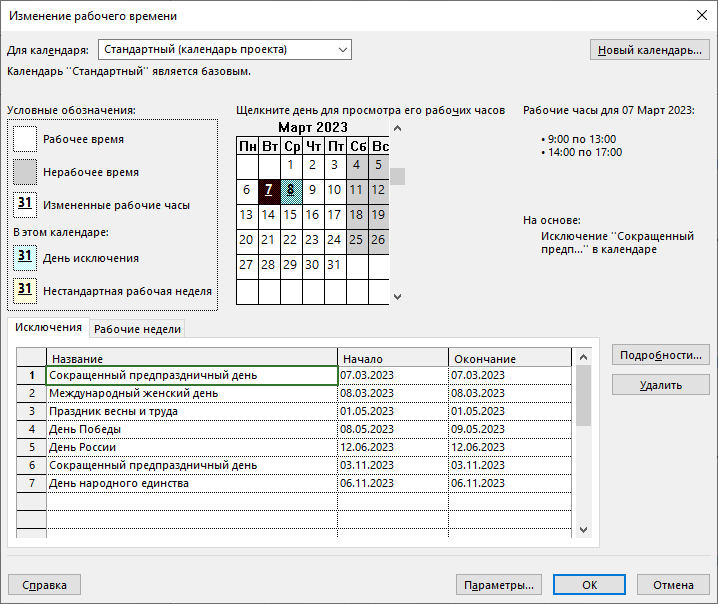
\includegraphics[width=\textwidth]{imgs/task_1_2.png}
	\end{center}
	\caption{Настройка нерабочих праздничных дней}
	\label{img:label}
\end{figure}

На вкладке \texttt{Задача -> Суммарная задача} установлена суммарная задача проекта и добавлена заметка с основной информацией о проекте.

\begin{figure}[H]
	\begin{center}
		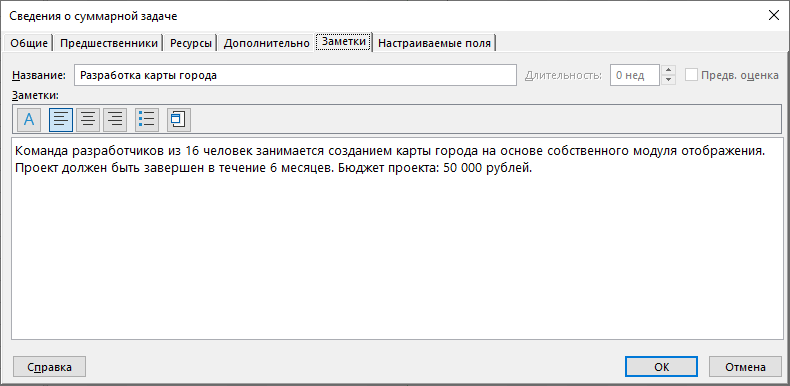
\includegraphics[width=\textwidth]{imgs/task_1_3.png}
	\end{center}
	\caption{Настройка суммарной задачи}
	\label{img:label}
\end{figure}

\section{Создание списка задач}

Осуществлен ввод задач с ручным планированием.

\begin{figure}[H]
	\begin{center}
		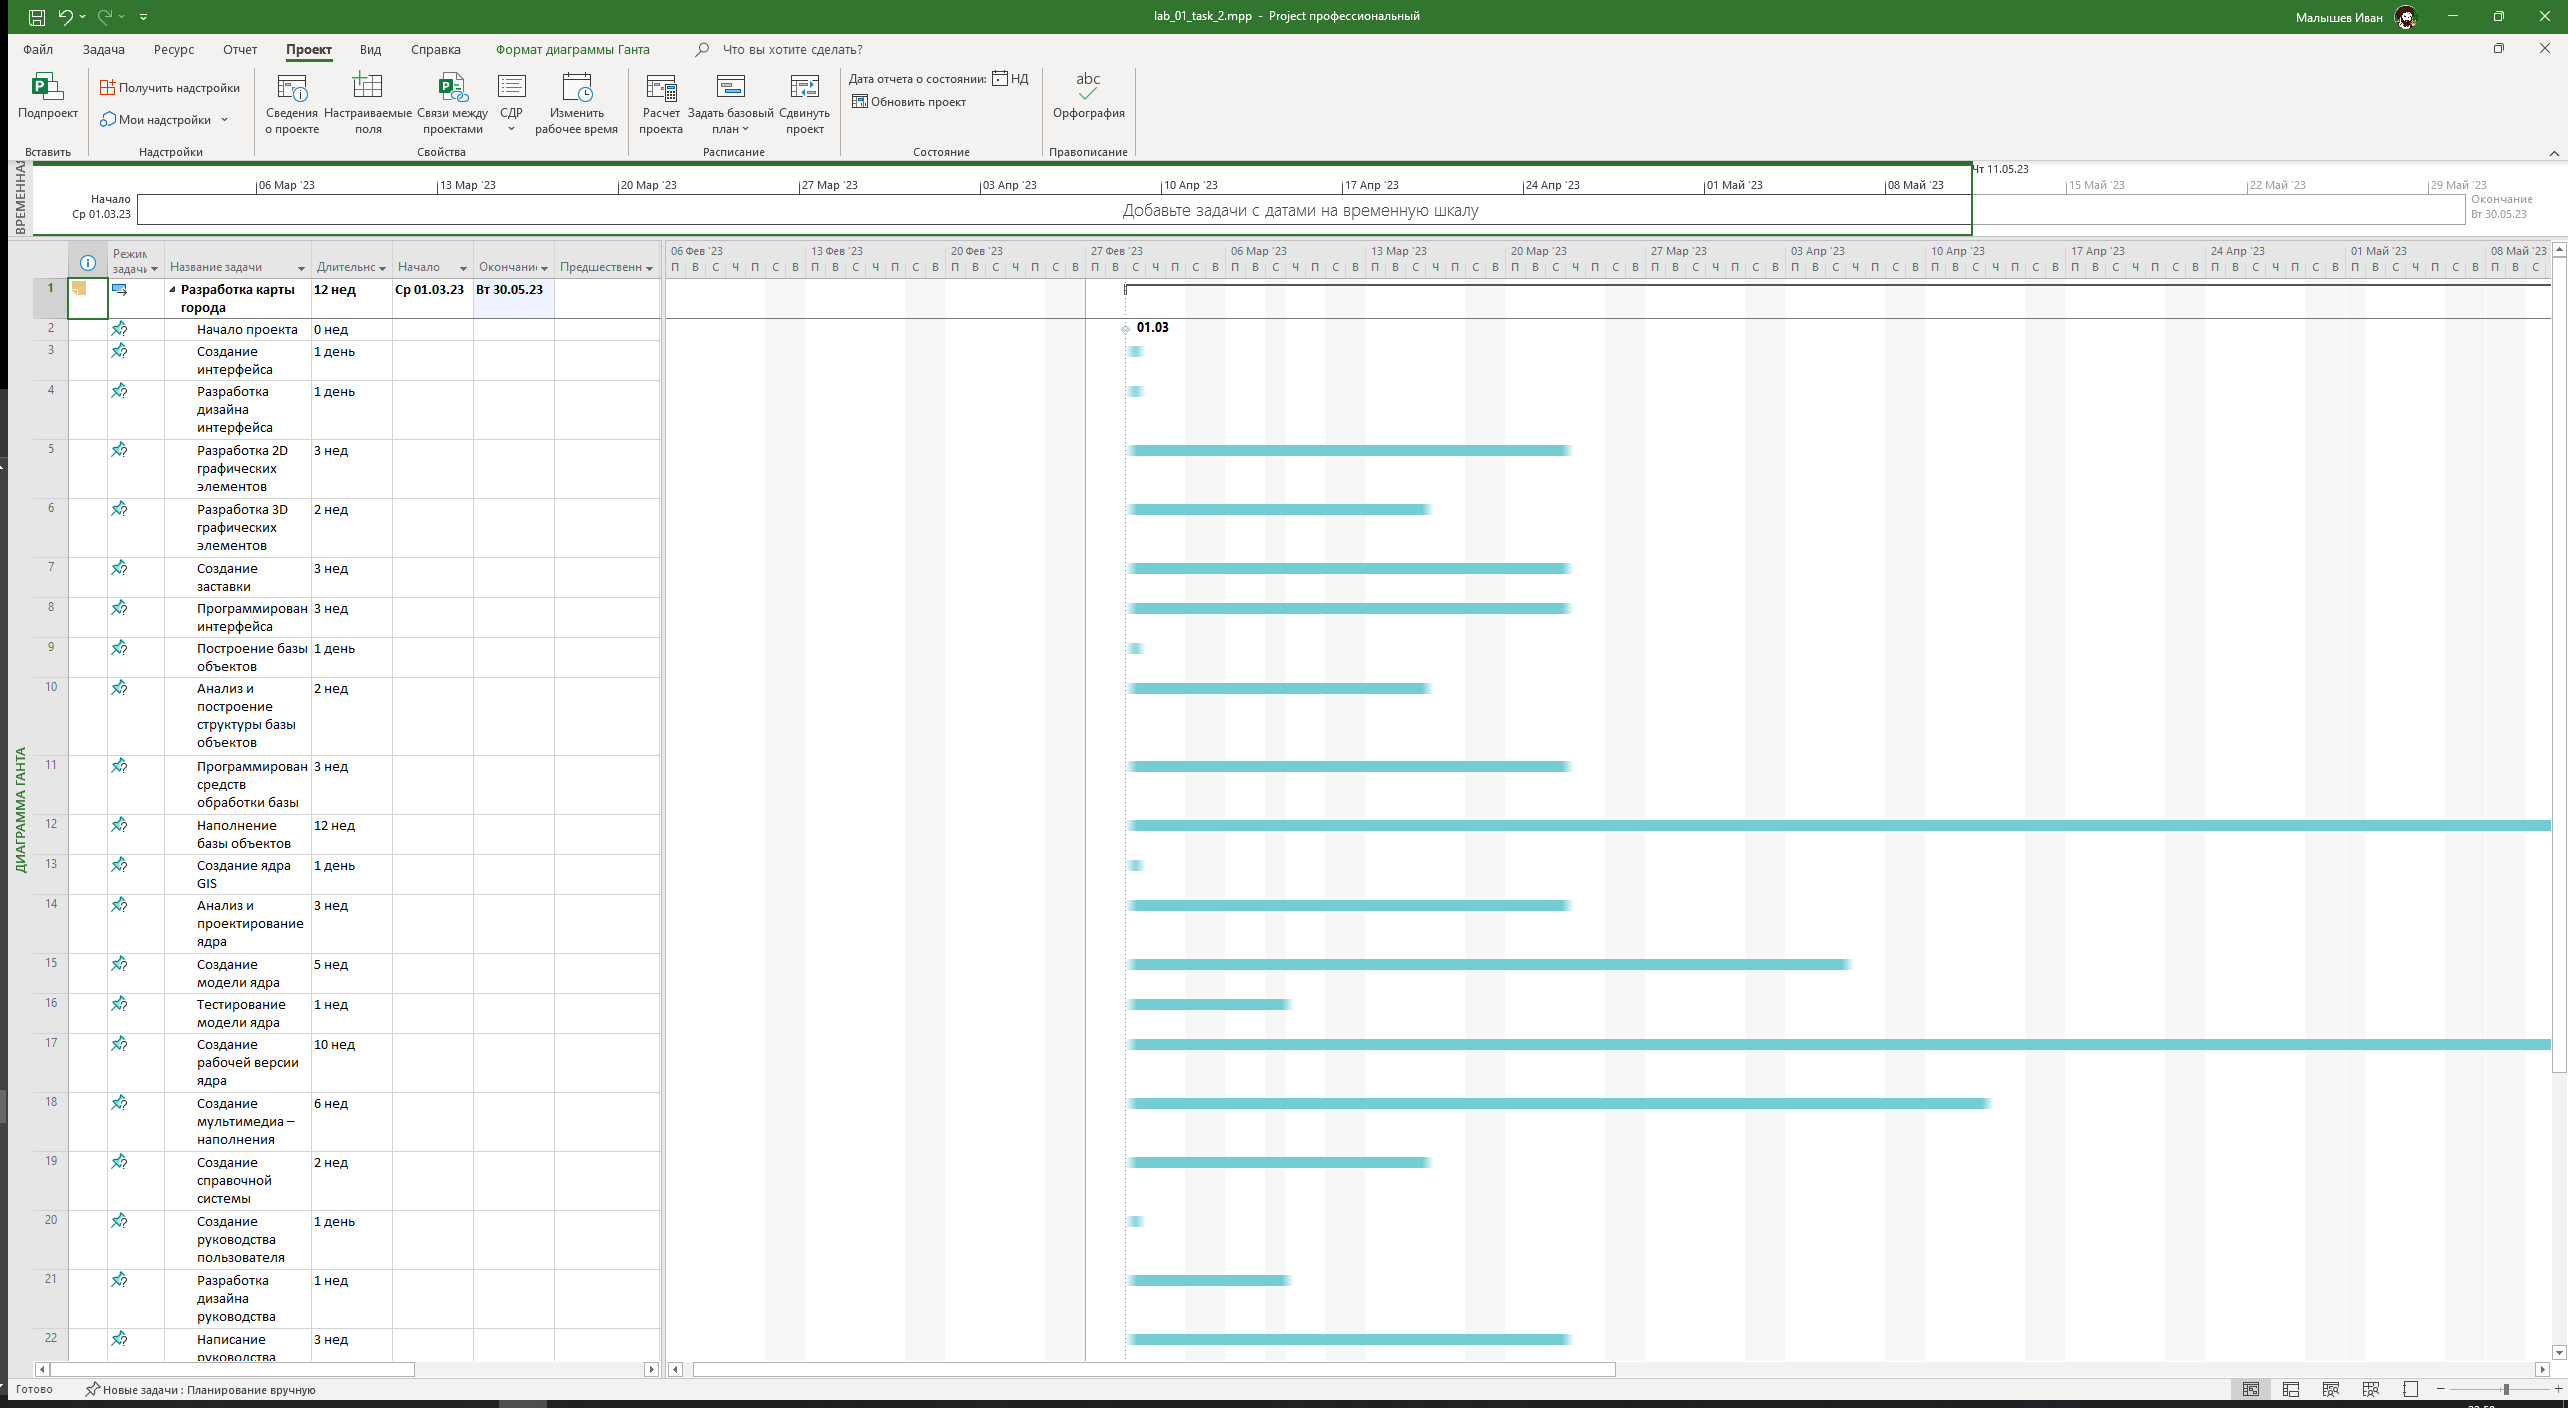
\includegraphics[width=\textwidth]{imgs/task_2_0.png}
	\end{center}
	\caption{Ввод задач}
	\label{img:label}
\end{figure}

\section{Структурирование списка задач}

При помощи кнопки \texttt{Понизить уровень задачи} были выделены подзадачи в соответствии с условием.

\begin{figure}[H]
	\begin{center}
		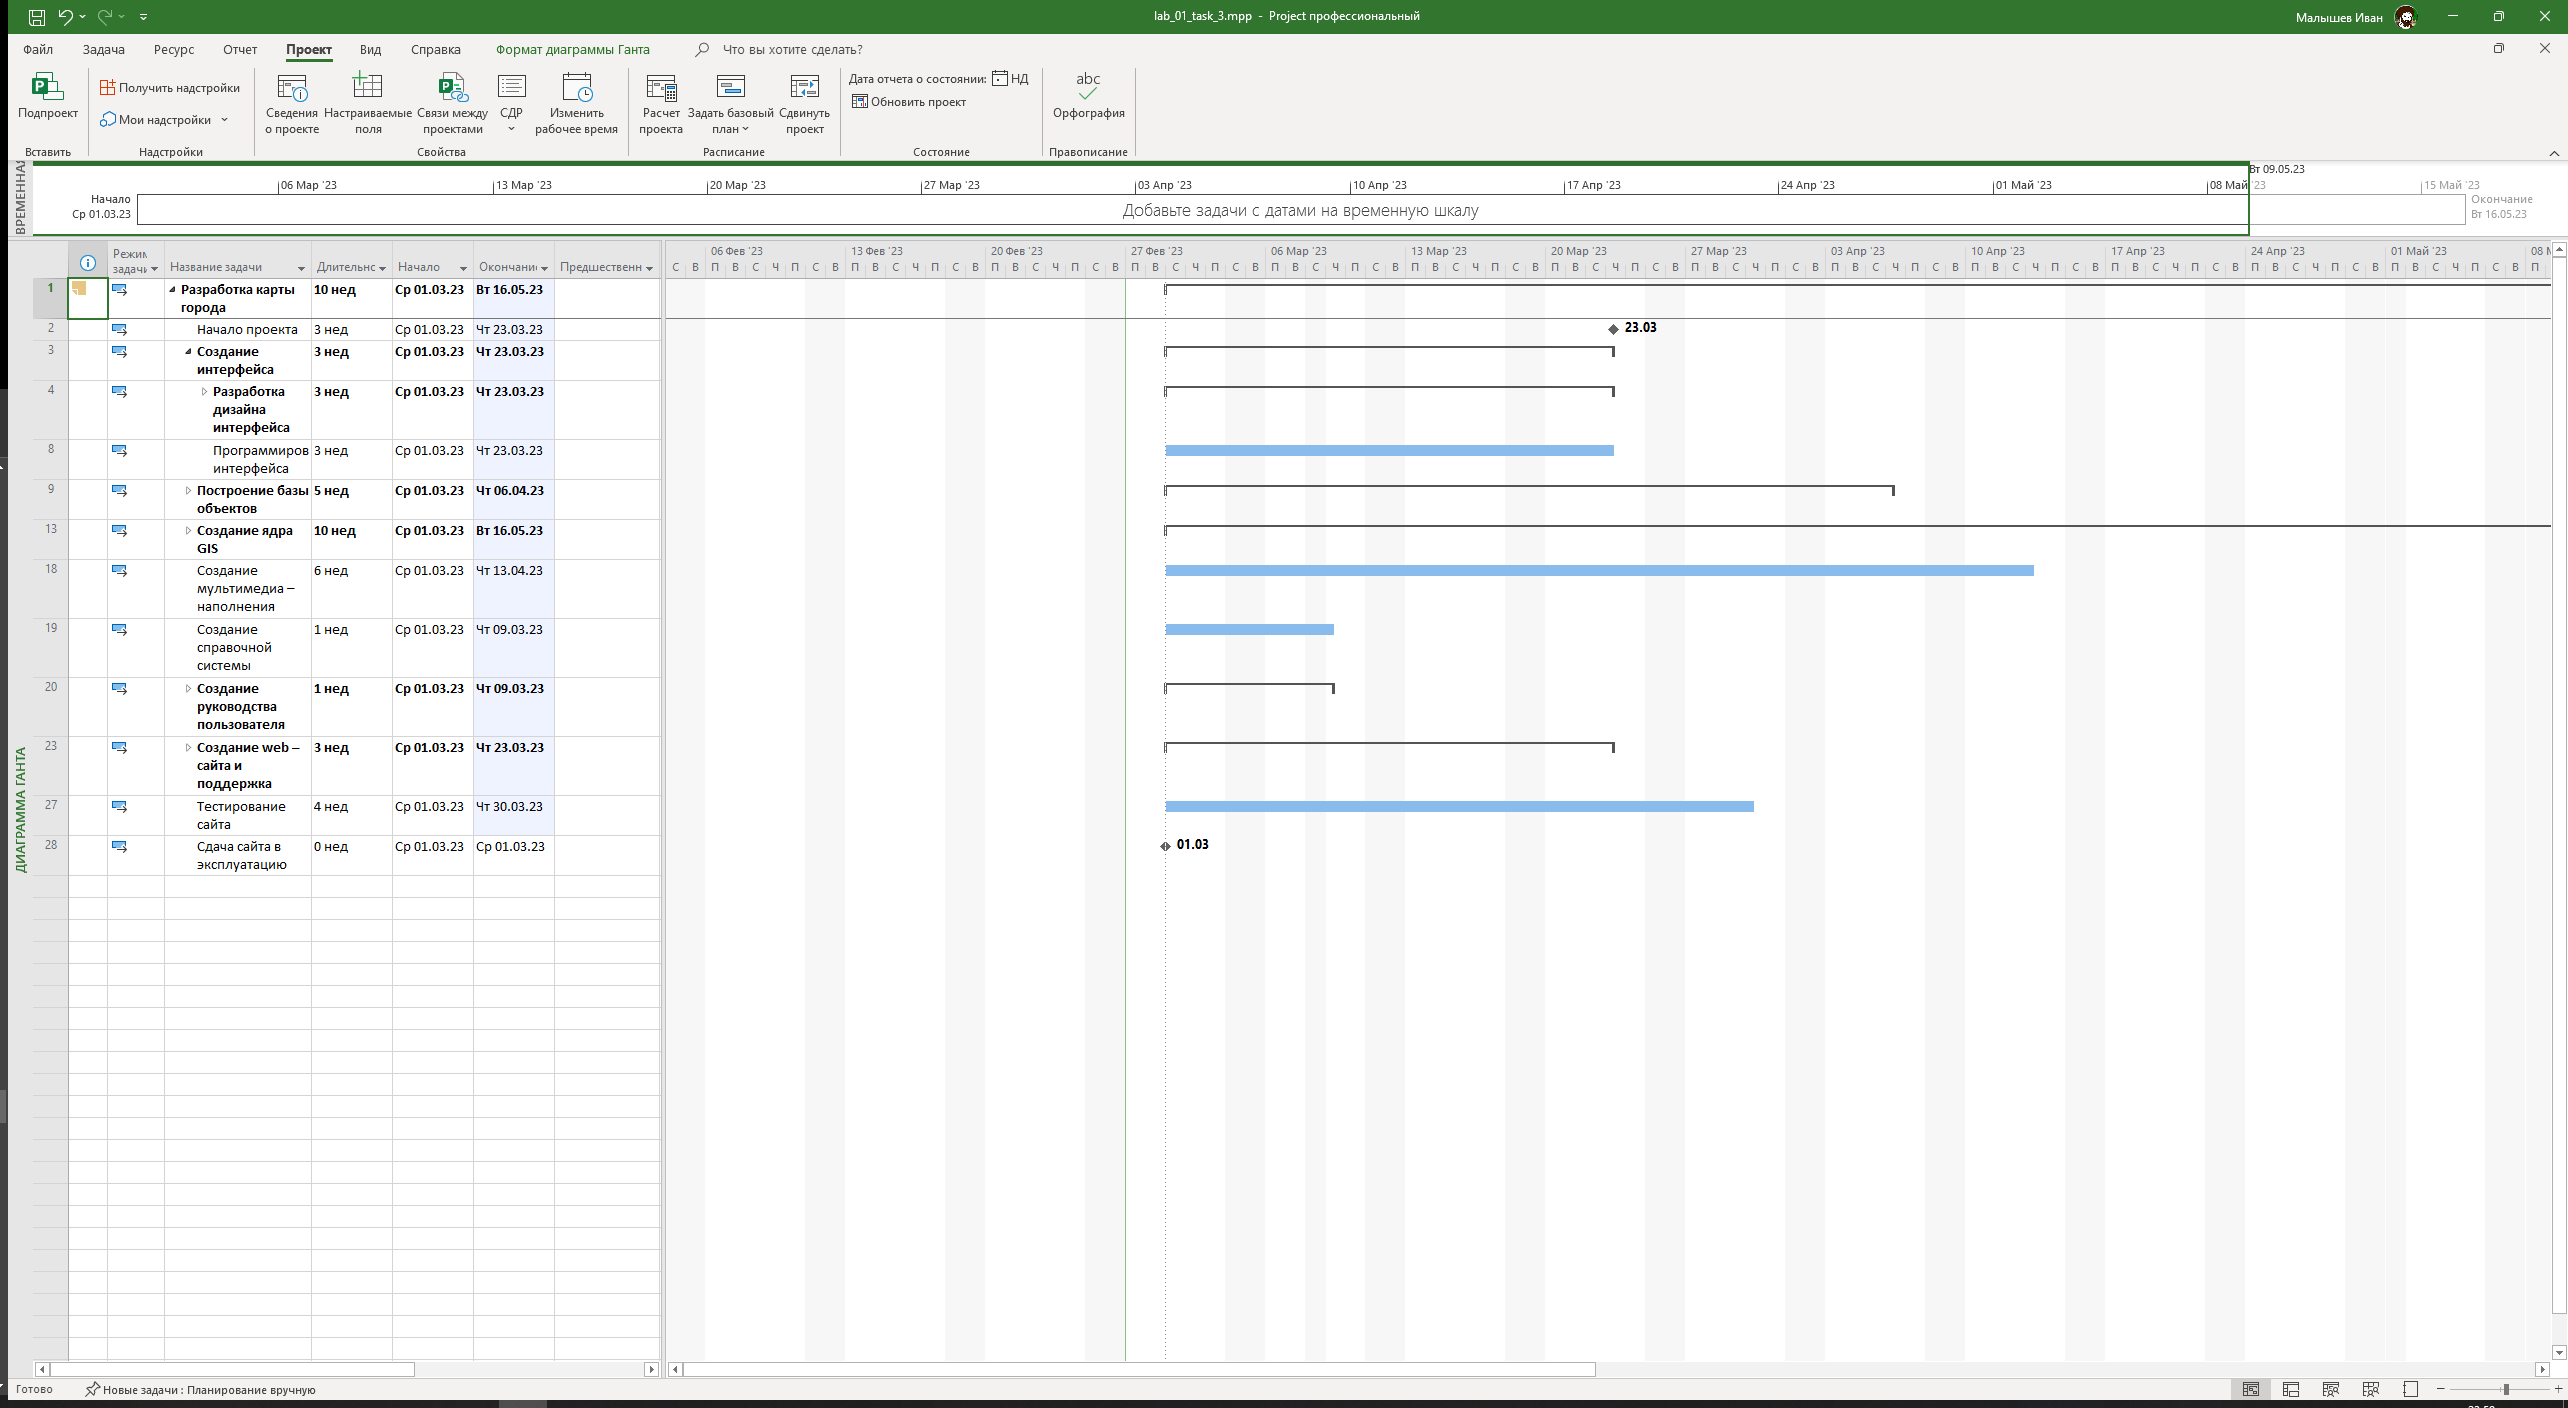
\includegraphics[width=\textwidth]{imgs/task_3_0.png}
	\end{center}
	\caption{Разбиение на подзадачи}
	\label{img:label}
\end{figure}

Также был установлен автоматический режим задач.

\section{Установление связей между задачами}

При помощи заполнения колонки \texttt{Предшественник} у каждой задачи были установлены связи между задачами.

\begin{figure}[H]
	\begin{center}
		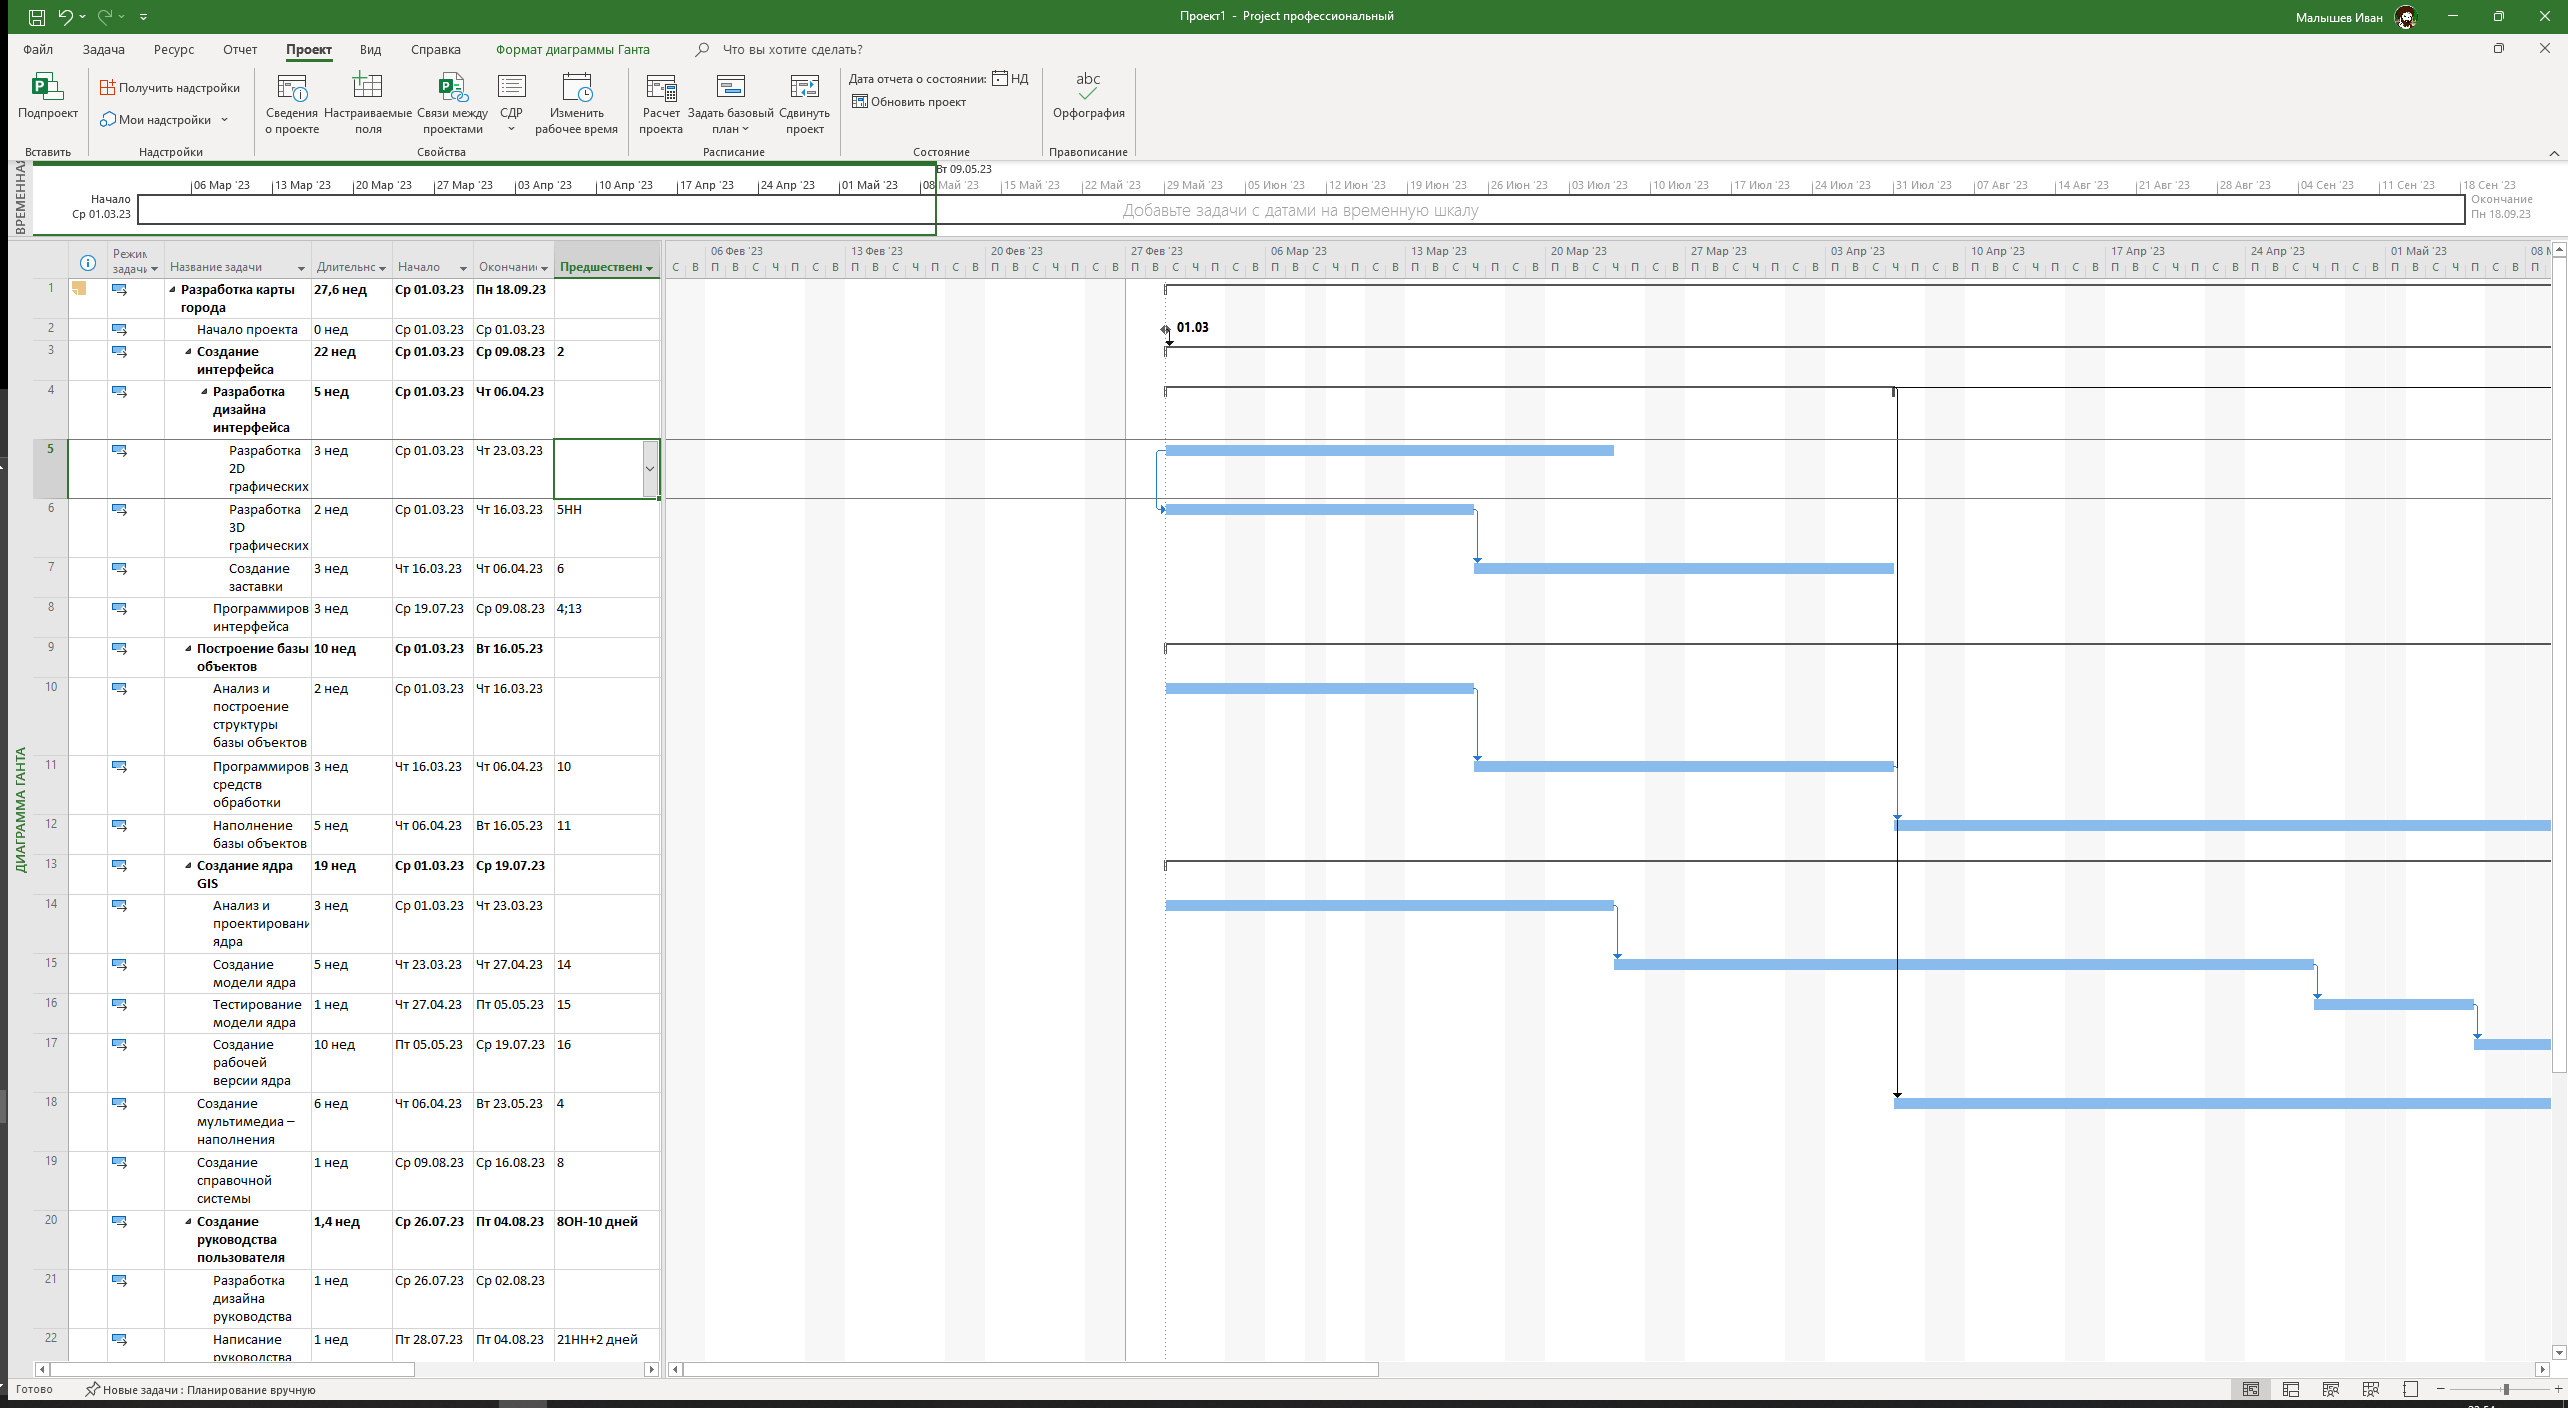
\includegraphics[width=\textwidth]{imgs/task_4_0.png}
	\end{center}
	\caption{Установленные связи между задачами}
	\label{img:label}
\end{figure}